% ----------------------------------------------------------------------------------------
% CHAPTER TITLE
% ----------------------------------------------------------------------------------------
\chapter{Selected Recent Works & Their Authors}\label{selrecworks}
\lhead{\chaptertitlename\ \thechapter. \emph{Selected Recent Works}}
% ----------------------------------------------------------------------------------------

This chapter describes a selection of designs from the past few years by makers in electronic music. These designs relate in many ways to the concept of open source as it was discussed in the last chapter, that is, devices which in their creation process create some amount of freely available information that enables future developers.

They were selected because they serve as examples of progress in a modern vision of electronic music hardware and its related approach to composition. Either through ideas or implementations, they constitute a compelling progress in the field. Documentation (either public, academic, or reverse-engineered) for these devices was collected and analyzed, and this chapter is a series of case studies explaining how these works were developed and why they are important in our context of open design. 

As will be detailed, broad categories are identified and used to group some of the projects. 

\section{Devi Ever FX and Dwarfcraft Devices}

Devi Ever FX was initially ran by a Devi Ever, who designed a long list of different distortion pedals before leaving the business to Louise and Ben Hinz. Devi was particularly appreciated in the online pedal DIY scene for her willingness to share and discuss audio circuit designs. 

One of these designs in particular appears as interesting: the \emph{improbability drive}. It was selected for the way this particular project is approached by community, and the ubiquitous role of fuzz pedals in the development of a diy practice. Paraphrasing an earlier citation from Collins, the internet did explode, and with it, a thousand fuzz designs did become available. For some, they were a way to waste time and money, for others, these became the foundation for multiple businesses. 

\subsection{the improbability drive (2011)}

Devi Ever (under the new Hinz ownership) currently sells 23 different designs of guitar effect pedals (mainly focused around distortions, overdrives or fuzzes), while its ``outdated'' page names 30 additional discontinued models. 

The Improbability Drive's circuit was first posted by Devi Ever herself on the freestompboxes.org forum, which is appreciated for its experienced reverse engineering community of musicians and experimenters. Although the original schematic is no longer available on the discussion thread, it was picked up by Ken Schurer of Infanem (Instruments for a New Electric Music, w2015), traced, and posted back by user B3ar on digi2t's request. 

	\begin{figure}[h!]
	  \caption{The Improbability Drive, traced from a second version board (courtesy of Ken Schurer)}
	  \centering
	    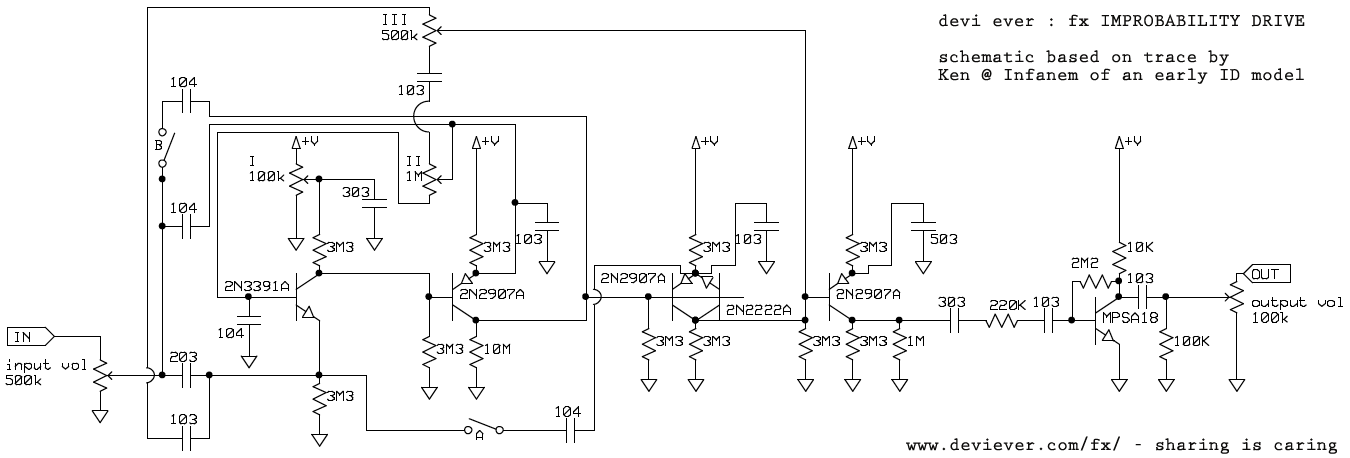
\includegraphics[width=.5\textwidth]{improbdr}
	\end{figure}
	
Following up on this project, user Storyboardist designed a proto-board and circuit board layout and shares it with the rest of the thread. Astrobass and digi2t discuss the finer details of the modifications Schurer might have made to Devi Ever's original design. 

	\begin{figure}[h!]
	  \caption{The Improbability Drive, layed out by storyboardist for proto-board and PCB}
	  \centering
	    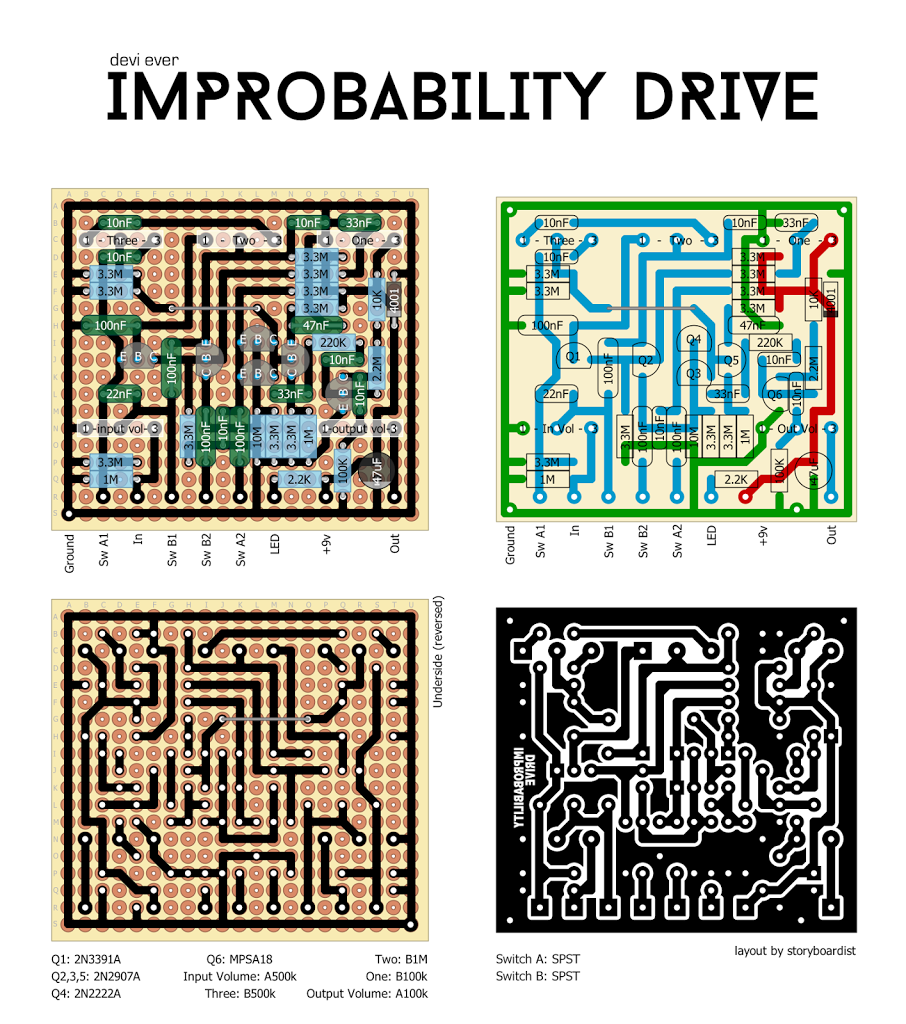
\includegraphics[width=.5\textwidth]{improbdr2}
	\end{figure}

In a couple of pages' worth of discussion, a discrete transistor fuzz circuit was resurected and made easily implementable by anyone with 15 dollars worth of parts and a few hours of time, for no reason other than users appreciated Ever's original contribution and were willing to entertain another user's delayed interest. Schurer, who originally retraced the design, sold a number of extra PCBs he had made in the process. 

This process is a typical maker practice, and constitutes the main source of content for websites like Hackaday, Instructables and portions of the Make website (as we'll see in a few sections). 

Other threads vary in detail. Some offer in-depth, component level analysis of each circuit, while other describe products so rare that there is barely any information on the topic. Unlike torrenting forums where rare catches are motivated by the concept of ratio bounty, users have little incentives to help other than curiosity and personal satisfaction. 

% add circuit analysis! 

This example shows two things: first, that open approaches in electronic music hardware is still present today, and, second, that those open practices are in effect accessible to anyone with the resources and time to learn how to read a schematic in proximity of a soldering iron. Introductory projects such as this have two other consequences: encouraging the development of more sophisticated, personal projects, and serving as an educational gateway to circuits and notions of electrical engineering, design, fabrication, and sometimes, patent law. 

``http://freestompboxes.org/viewtopic.php?f=7&t=18157&hilit=devi+ever+fx''

\section{CMOS synthesis: modern incarnations}

All the transistors in the improbability drive are high power, low noise NPN small signal silicon bipolar junction transistors (BJT), which is what could be expected from a discrete audio circuit  design. 

However, as the following chapter will describe, electronic music instrument design is shaped by a pragmatism for achieving a specific goal with simple and clever circuits. Musical and hardware subcultures are sometimes based upon specific approaches to those circuits \citep{ghazala2005,collins2006,hegarty2007,novak2013}. Of these approaches, the following appears to have had a significant importance in the development of expressive audio electronics while questioning the boundary between utilitarian and artistic, analog and digital. 


\begin{quote}
	
	We can make our ``1"-``0" decisions into just about anything- a musical note, a test waveform, a measured and displayed value, a video presentation, a clock, a game, an industrial control, a toy, a microcomputer, an art form, a community information access service, or just about anything else you can dream up. All it takes is the right number of logic blocks properly connected to do the job.
	\citep[pp-7-8]{lancaster1988}
	
\end{quote}

\emph{Handmade Electronic Music} focuses much of its circuits around the Complementary-Silicon-Metal-Oxide (CMOS) family of integrated circuits. He acknowledges inspiration from Lancaster's CMOS cookbook, quoted above (personal conversation, 2015). In doing so, Collins acknowledges how powerful binary signals - an its continuous counterpart, the square wave - can be in relatively simple synthesis environments. Older examples abound: the Weird Sound Generator, a typical first synthesis project sold as a kit by Ray Wilson from the \emph{Music From Outer Space} website, relies on interconnected CMOS chips for its synthesis \citep{wilson2015}. Beavis Audio, an important diy music website, focuses one of its most interesting blog posts on this family of circuits, naming Collins as an influence \citep{beavis2015}. 

Although Collins is not the only source of these digital logic sound generators, the publication of his book has had a visible impact on many of the low-part-count synthesis circuits seen today. The two following examples exhibit particularly interesting and relevant projects, all ``open'' to some extent. 

\subsection{Dwarfcraft: the Robot Devil (2012)}

The relative simplicity of the device is here extremely relevant, as it has lead online community members to relate it to some circuits described in Nic Collins' \emph{Handmade Electronic Music}. 

``http://freestompboxes.org/viewtopic.php?f=7&t=18344&hilit=robot+devil''

The power of CMOS logic chips also serves as a segway into the wider topic of microcontroller synthesis. If Tristan Shone's system exhibited the power of arduinos in the context of controllers, numerous practitioners have also been developing instruments  In this case, embedded systems of various complexity have been used in innumerable synthesis projects, providing low fidelity audio outputs and high potential for customization. Sonically, these projects are very much indebted to the auditory product of CMOS chips combined with basic filtering and effects. 

\subsection{Taylan Cihan: Porcupine (2013)}

\begin{quote}
	
	After being stabbed numerous times by the wires sticking out of the device while building it, the name, Porcupine, came out rather naturally. Porcupine, as I would like call, is a concrète box (in reference to musique concrète), combining a built-in analog sound processor with a variety of acoustic sounds that can be generated using the wires. The copper plate and wires are essentially leftover parts from my previous project, Vermes. Instead of throwing it all away, I have decided to recycle them, hence the faint artwork on the surface of the plate, a by-product of my failed very first attempt at making my own PCB.

	The sound processor include an analog delay, fuzz distortion, and resonating low-pass filter. A piezo element attached to the copper plate picks up the sound of the wires, which is amplified through a high-gain preamp before sent to the processing unit. An additional 1/4" jack input, which also has its own high-gain preamp, allows the device to be simultenously used as an effects unit to process the external sounds. When the levels, delay time, fuzz gain and filter resonance set to a maximum, the circuit starts to self-oscillate, producing a rich harmonic spectrum.
	
	\end{quote}
	
	\citep{cihan2015}
	

Taylan Cihan's porcupine device is important because it is typical of experimenters who've grown comfortable with the various components of standard circuits such as those presented in \emph{Handmade Electronic Music}. Experiments with higher-level design and adapting interfaces are often the first step to making more compelling instruments: in this case, this is achieved by combining semi-standard circuits and by turning the design of an interface inside out to embrace the chaotic experiments from which it came. 

Specifically, Cihan's circuit is based on the following building blocks: 
	
\begin{quote}
		
The delay unit is built using a PT2399 Echo Processor IC by Princeton Technologies.

Fuzz distortion is a clone of EHX Muff Fuzz. Schematic from Beavis Audio.

The 4049 Hex Inverter preamp schematic is from Nick Collins' Handmade Electronic Music book (p.187).
	
	\end{quote}

	\citep{cihan2015}

	\begin{figure}[h!]
	  \caption{Cihan's \emph{Porcupine}, front view}
	  \centering
	    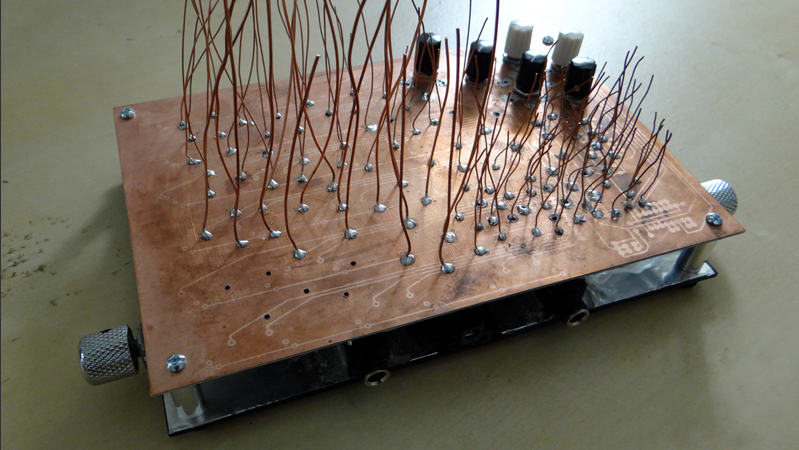
\includegraphics[width=.5\textwidth]{porcupinetop}
	\end{figure}
	
	\begin{figure}[h!]
	  \caption{Cihan's \emph{Porcupine}, circuit board view}
	  \centering
	    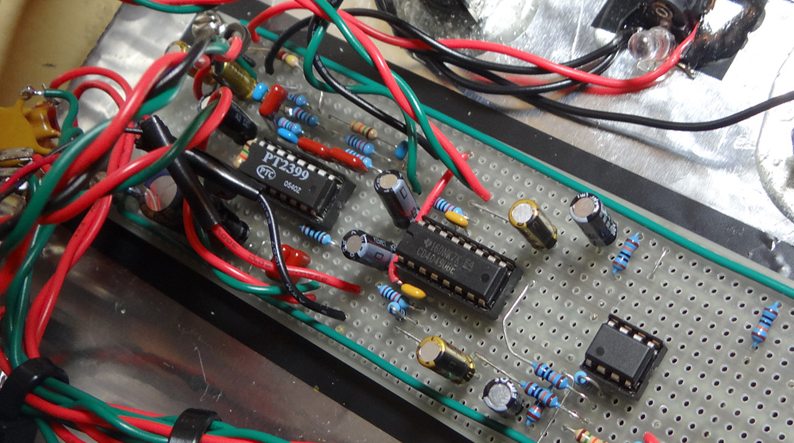
\includegraphics[width=.5\textwidth]{porcupinein}
	\end{figure}
	
The circuit board view shows three integrated circuits: a PT2399, a 4049, and a eight pin DIP package IC.

The 4049 is a CMOS Hex Inverter used as a resonating low pass filter, based on one of Nic Collins' designs.

	\begin{figure}[h!]
	  \caption{Nic Collins' 4049 Low Pass Resonating filter from \emph{Handmade Electronic Music}}
	  \centering
	    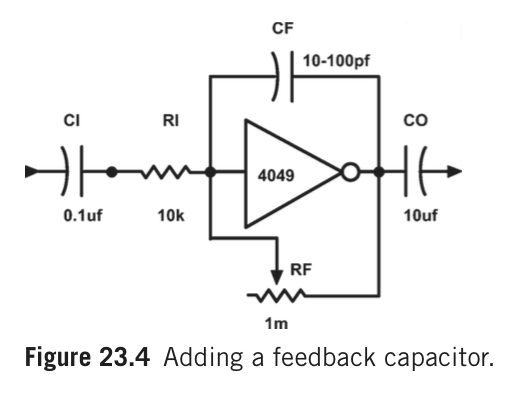
\includegraphics[width=.5\textwidth]{4049lpf}
	\end{figure} 
	
As detailed in the previous chapter, this circuit and its associated notes are available in the public draft for \emph{Hardware Hacking}. 

	\begin{figure}[h!]
	  \caption{Nic Collins' 4049 Low Pass Resonating filter from \emph{Hardware Hacking}}
	  \centering
	    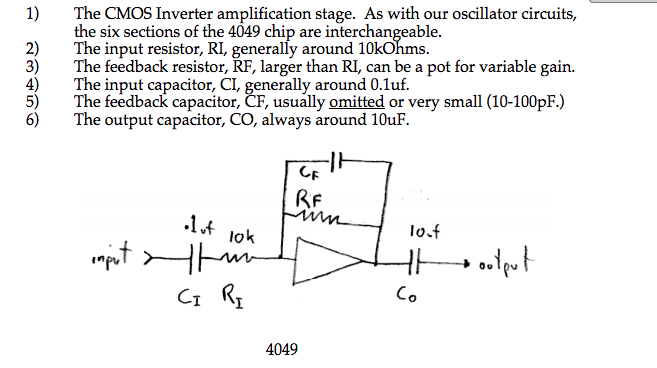
\includegraphics[width=.5\textwidth]{4049lpf2}
	\end{figure} 

The PT2399, with two electrolytic capactitors, seven mylar capacitors and eight resistors, appears to be a variation on the stock circuit from the PT2399 application note.

	\begin{figure}[h!]
	  \caption{PT2399 stock circuit, from the application note by Princeton Technologies}
	  \centering
	    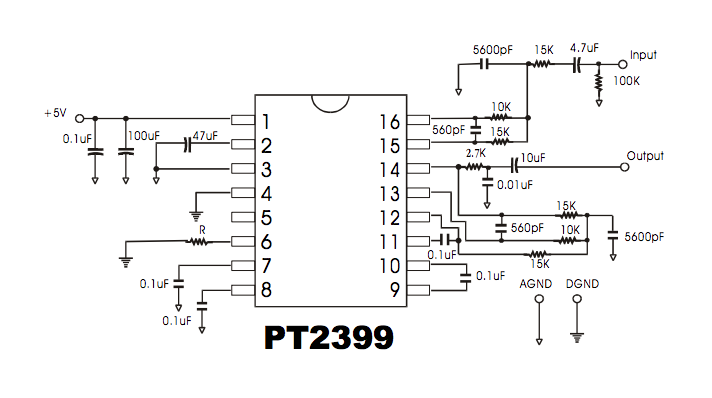
\includegraphics[width=.5\textwidth]{pt2399circ}
	\end{figure}
	
The Muff fuzz circuit is based on an original Electro-Harmonix design as traced by Beavis Audio. It is a classic of distortion circuits, a simple and expressive two transistor design which gave Electro Harmonix its reputation. Its parts are common and inexpensive, with various diy vendors offering kit versions with extremely detailed assembly instructions.

	\begin{figure}[h!]
	  \caption{Beavis Audio Muff Fuzz}
	  \centering
	    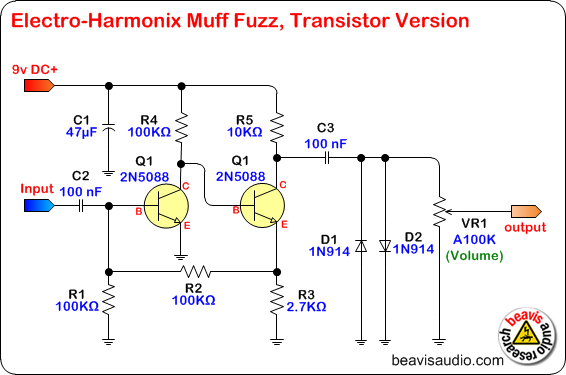
\includegraphics[width=.5\textwidth]{mufffuzzbeavis}
	\end{figure}
	
The third chip, although illegible in the picture above, is probably an op-amp IC used for the piezo preamp Cihan mentions. 

In effect, this combination of circuits and hardware is a versatile, expressive and personal approach to exploring the possibilities of audio circuits. It is simple enough to be understood in two paragraphs, two links and one reference, but the result is arguably greater than the sum of its parts. This is especially due to the nature of the interface, the ability of the device to both process and generate, and the re-use of materials from a previous project. By exposing the mess of wires and their prickly unfriendliness, Cihan exhibits his clear appreciation for his medium of choice.

This is also where hardware design can ask greater questions in the field of music performance and sound art. The sculptural aspect of the device is indirectly reminiscent of sonic installations by Tudor, Lucier and their aesthetic descendants.\emph{Porcupine}'s ability to both generate and process sounds greatly enhances its potential to be part of a larger, evolving system. By sharing this design, Cihan quietly kept experimental ideals alive. By keeping the information incomplete, he also encouraged exploration and personalization: in effect, Cihan and his peers allow for open musical hardware to go from self-sustaining to self-expanding. 

It is interesting to note that Cihan detailed the PT2399 delay chip as an analog one. Indeed, the Princeton Technology Corporation datasheet identifies it as an ``echo audio processor IC utilizing CMOS technology which is equipped with ADC and DAC, high sampling frequency and an internal memory of 44k.'' \citep{princetonpt} The chip is occasionally labeled as analog (sounding convincingly so) by various manufacturers and diy guides - this suggests that Cihan gathered information from other experimenters online, making him a willing actor of these open practices. 
 
\section{microcomputer systems}

The PT2399 chip — a CMOS, digital sampling IC — is a good example of what followed basic logical operators of the 4000 series. 

	\begin{figure}[h!]
	  \caption{the PT2399 internal block diagram from the Princeton datasheet}
	  \centering
	    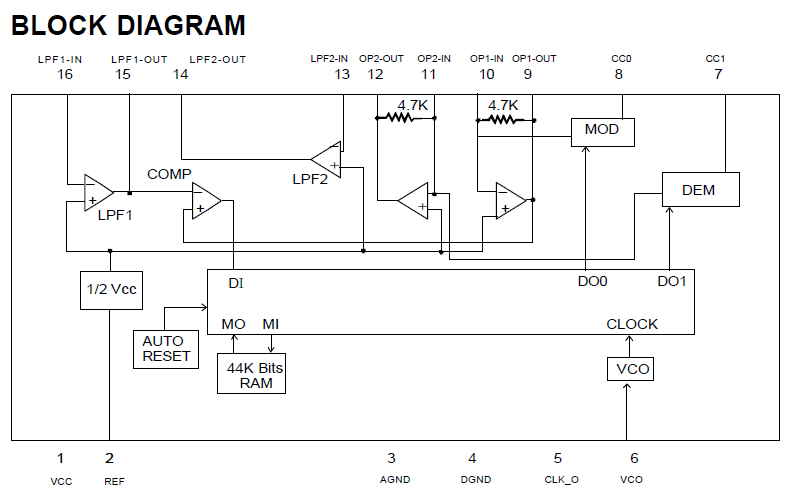
\includegraphics[width=.5\textwidth]{pt2399diag}
	\end{figure}

By combining large numbers of microscopic scale logical operators and connecting those to memories and clocks, CMOS sampling ICs such as this one are possible. The main limitation here is the relatively straightforward set of applications: generating delayed copies of the input signal. 

As other subcomponents of computing systems followed in the process of miniaturization, small and accessible systems have become ubiquitous in the arts because of their versatility \citep{gibb2010}.

	\begin{figure}[h!]
	  \caption{the AVR system block diagram for the ATMega328, from Atmel - included in the recent Arduino packages}
	  \centering
	    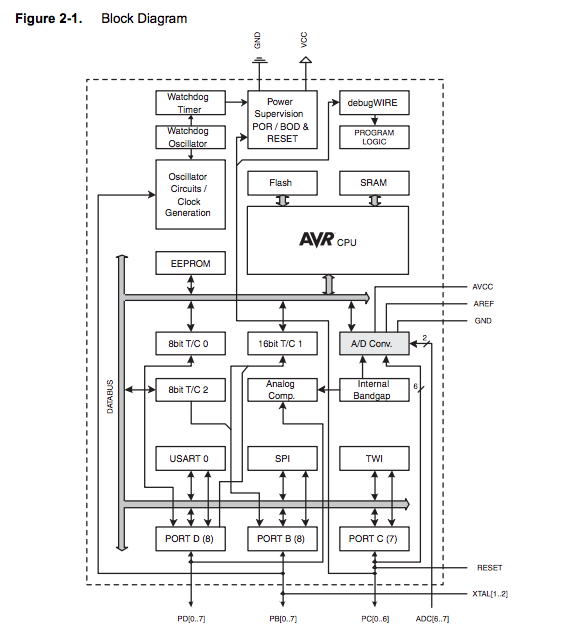
\includegraphics[width=1\textwidth]{avrarch}
	\end{figure}

In recent years, the family of arduino packages have had a particularly strong impact on creative computing in sound and installation work. Presenting those will also allow us to discuss instruments designed with slightly less user-friendly systems such as the ARM architecture in Martin Howse' \emph{Dark Interceptors} series.  

%add nic collins paper on computing 
 
%book about mainframe computer art? 

\subsection{Tristan Shone: Author and Punisher}

The first example of a musical practice based around microcontrollers is that of an artist going under the name \emph{Author and Punisher}. 

A mechanical engineer and sculptor, Tristan Shone is the musician responsible for this one-man project. He released a first album in 2005, \emph{The Painted Army} \citep{shone,2005}, as he was developing his first set of instruments, the Drone machines. His website's subtitle is ``electromechanical destruction since 2004'' \citep{shone2004}.

	\begin{figure}[h!]
	  \caption{Shone's live setup around the release of the \emph{Drone Machines} album}
	  \centering
	    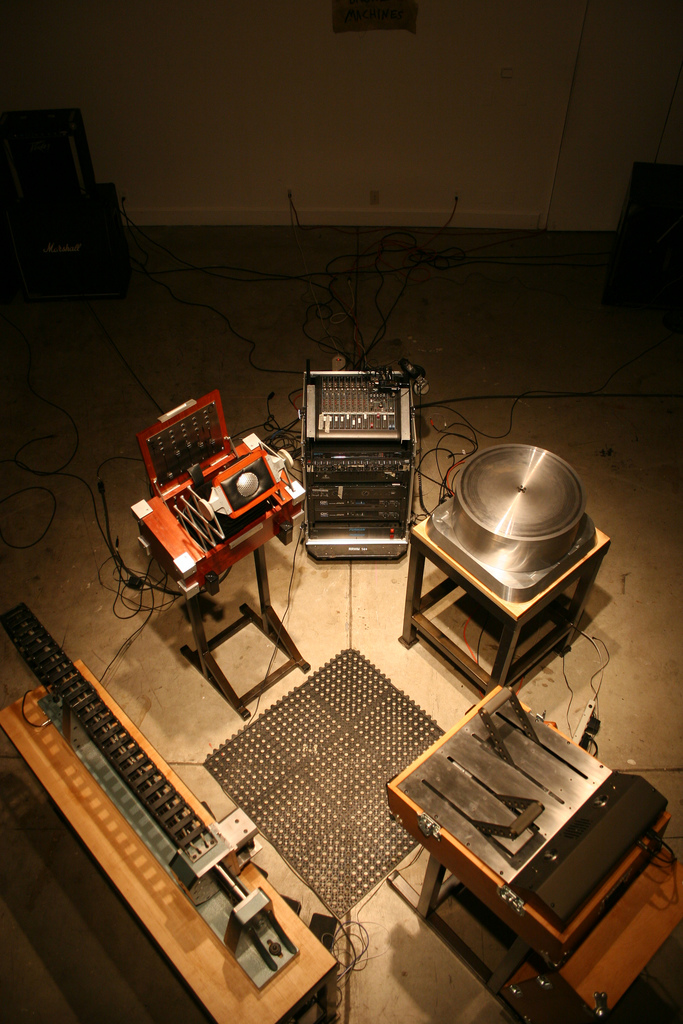
\includegraphics[width=.5\textwidth]{drone}
	\end{figure}
	
He has since released three more full-lengths relying increasingly on hardware he fabricated, in conjunction with a software sampling and synthesis system built around Ableton Live. Most of his devices have evocative names such as \emph{Linear Actuator}, \emph{Big Knobs} or \emph{Bellows}. 

	\begin{figure}[h!]
	  \caption{the \emph{Linear Actuator}}
	  \centering
	    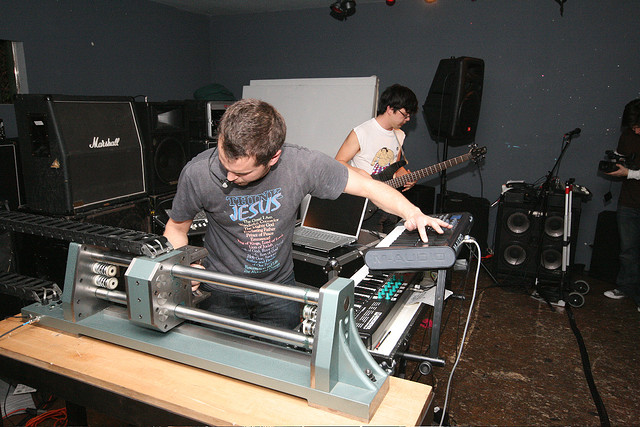
\includegraphics[width=1\textwidth]{linact}
	\end{figure}

	\begin{figure}[h!]
	  \caption{the \emph{Bellows}}
	  \centering
	    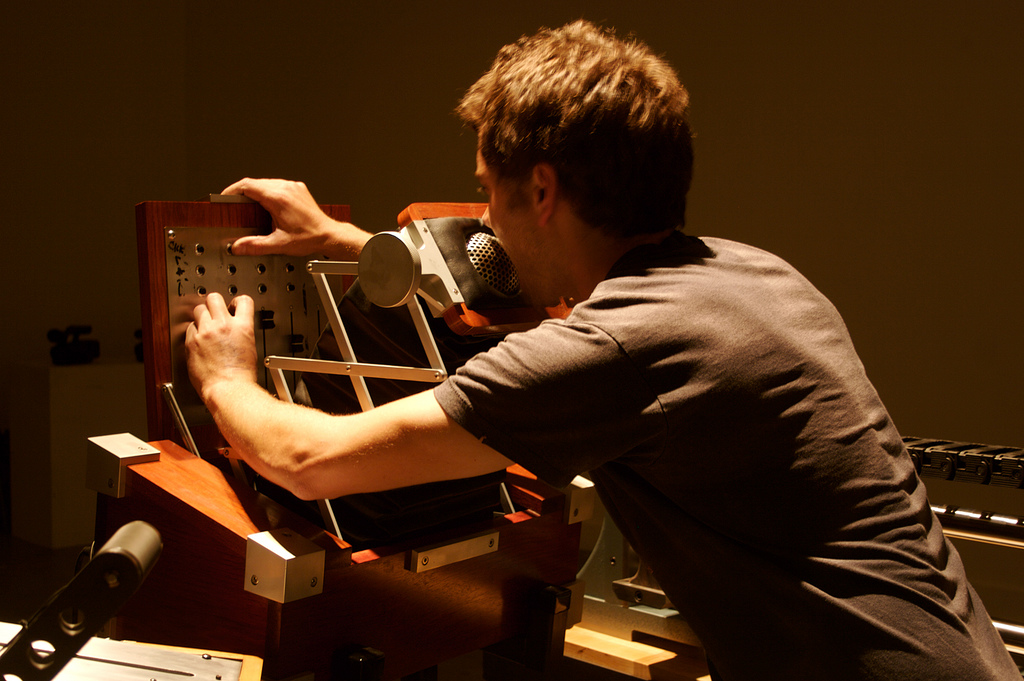
\includegraphics[width=1\textwidth]{bellows}
	\end{figure}

His experience with sculpture and mechanical engineering are clear, although discussing the matter with him makes it clear that he is ultimately making those because they seem like the best way to perform his music. Although he has grown to try and move away from the visual impact of his setup by collaborating with visual artists, his website still provides the curious with a combination of evocative live shots and technical diagrams. 

	\begin{figure}[h!]
	  \caption{a technical diagram for the \emph{Bellows} instrument}
	  \centering
	    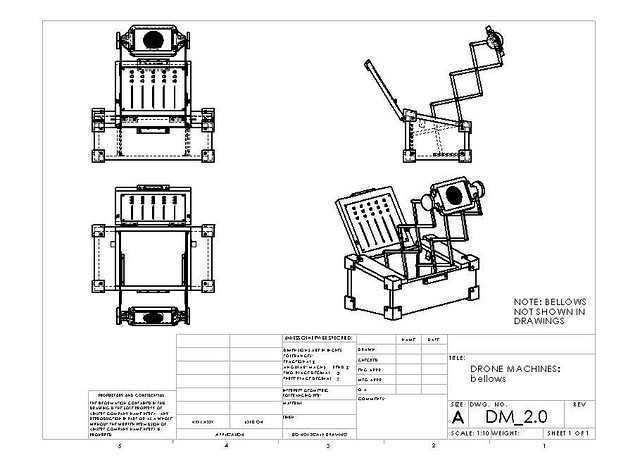
\includegraphics[width=1\textwidth]{bellowsdiag}
	\end{figure}
	
Most of these electromechanical devices act as controllers: they encode movement into a number using arduino systems. This information is then fed into a computer, which triggers starts, changes and ends for specific sets of pre-composed sounds. 

Shone's microcontroller system is based on the arduino environment, which he uses with custom firmware developed by Dimitri Diakopoulos and featured at NIME in 2011 \citep{diakopoulos2011,diakopoulos2015} . This firmware modification turns a specific strands of the Arduino hardware (the Uno, Due and Mega 2560 boards) into a driverless device, enabling it to send MIDI data over USB without any more setup than a commercial USB-MIDI item. 

However, Shone's live setup is not just centered around controllerism. Shone describes himself as a ``lifelong beatboxer'' and in this context, he's devised a number of ways to detect, record and manipulate his voice \citep{shone2012}. He's currently developing a set of masks (documented on his website are the trachea quad mic, the dither mask, the drone mask and the mute mask), while his previous vocal interface is called the Headgear. That system was the topic of a tutorial written by Shone for the Make Magazine website \citep{shone2012}. 

http://makezine.com/magazine/make-22/seriously-heavy-metal/

\paragraph{The Headgear system (2011)}

https://makezine.com/Project/Headgear-MIDI-Control/1206/1/

	\begin{figure}[h!]
	  \caption{the Headgear device, wired for operation}
	  \centering
	    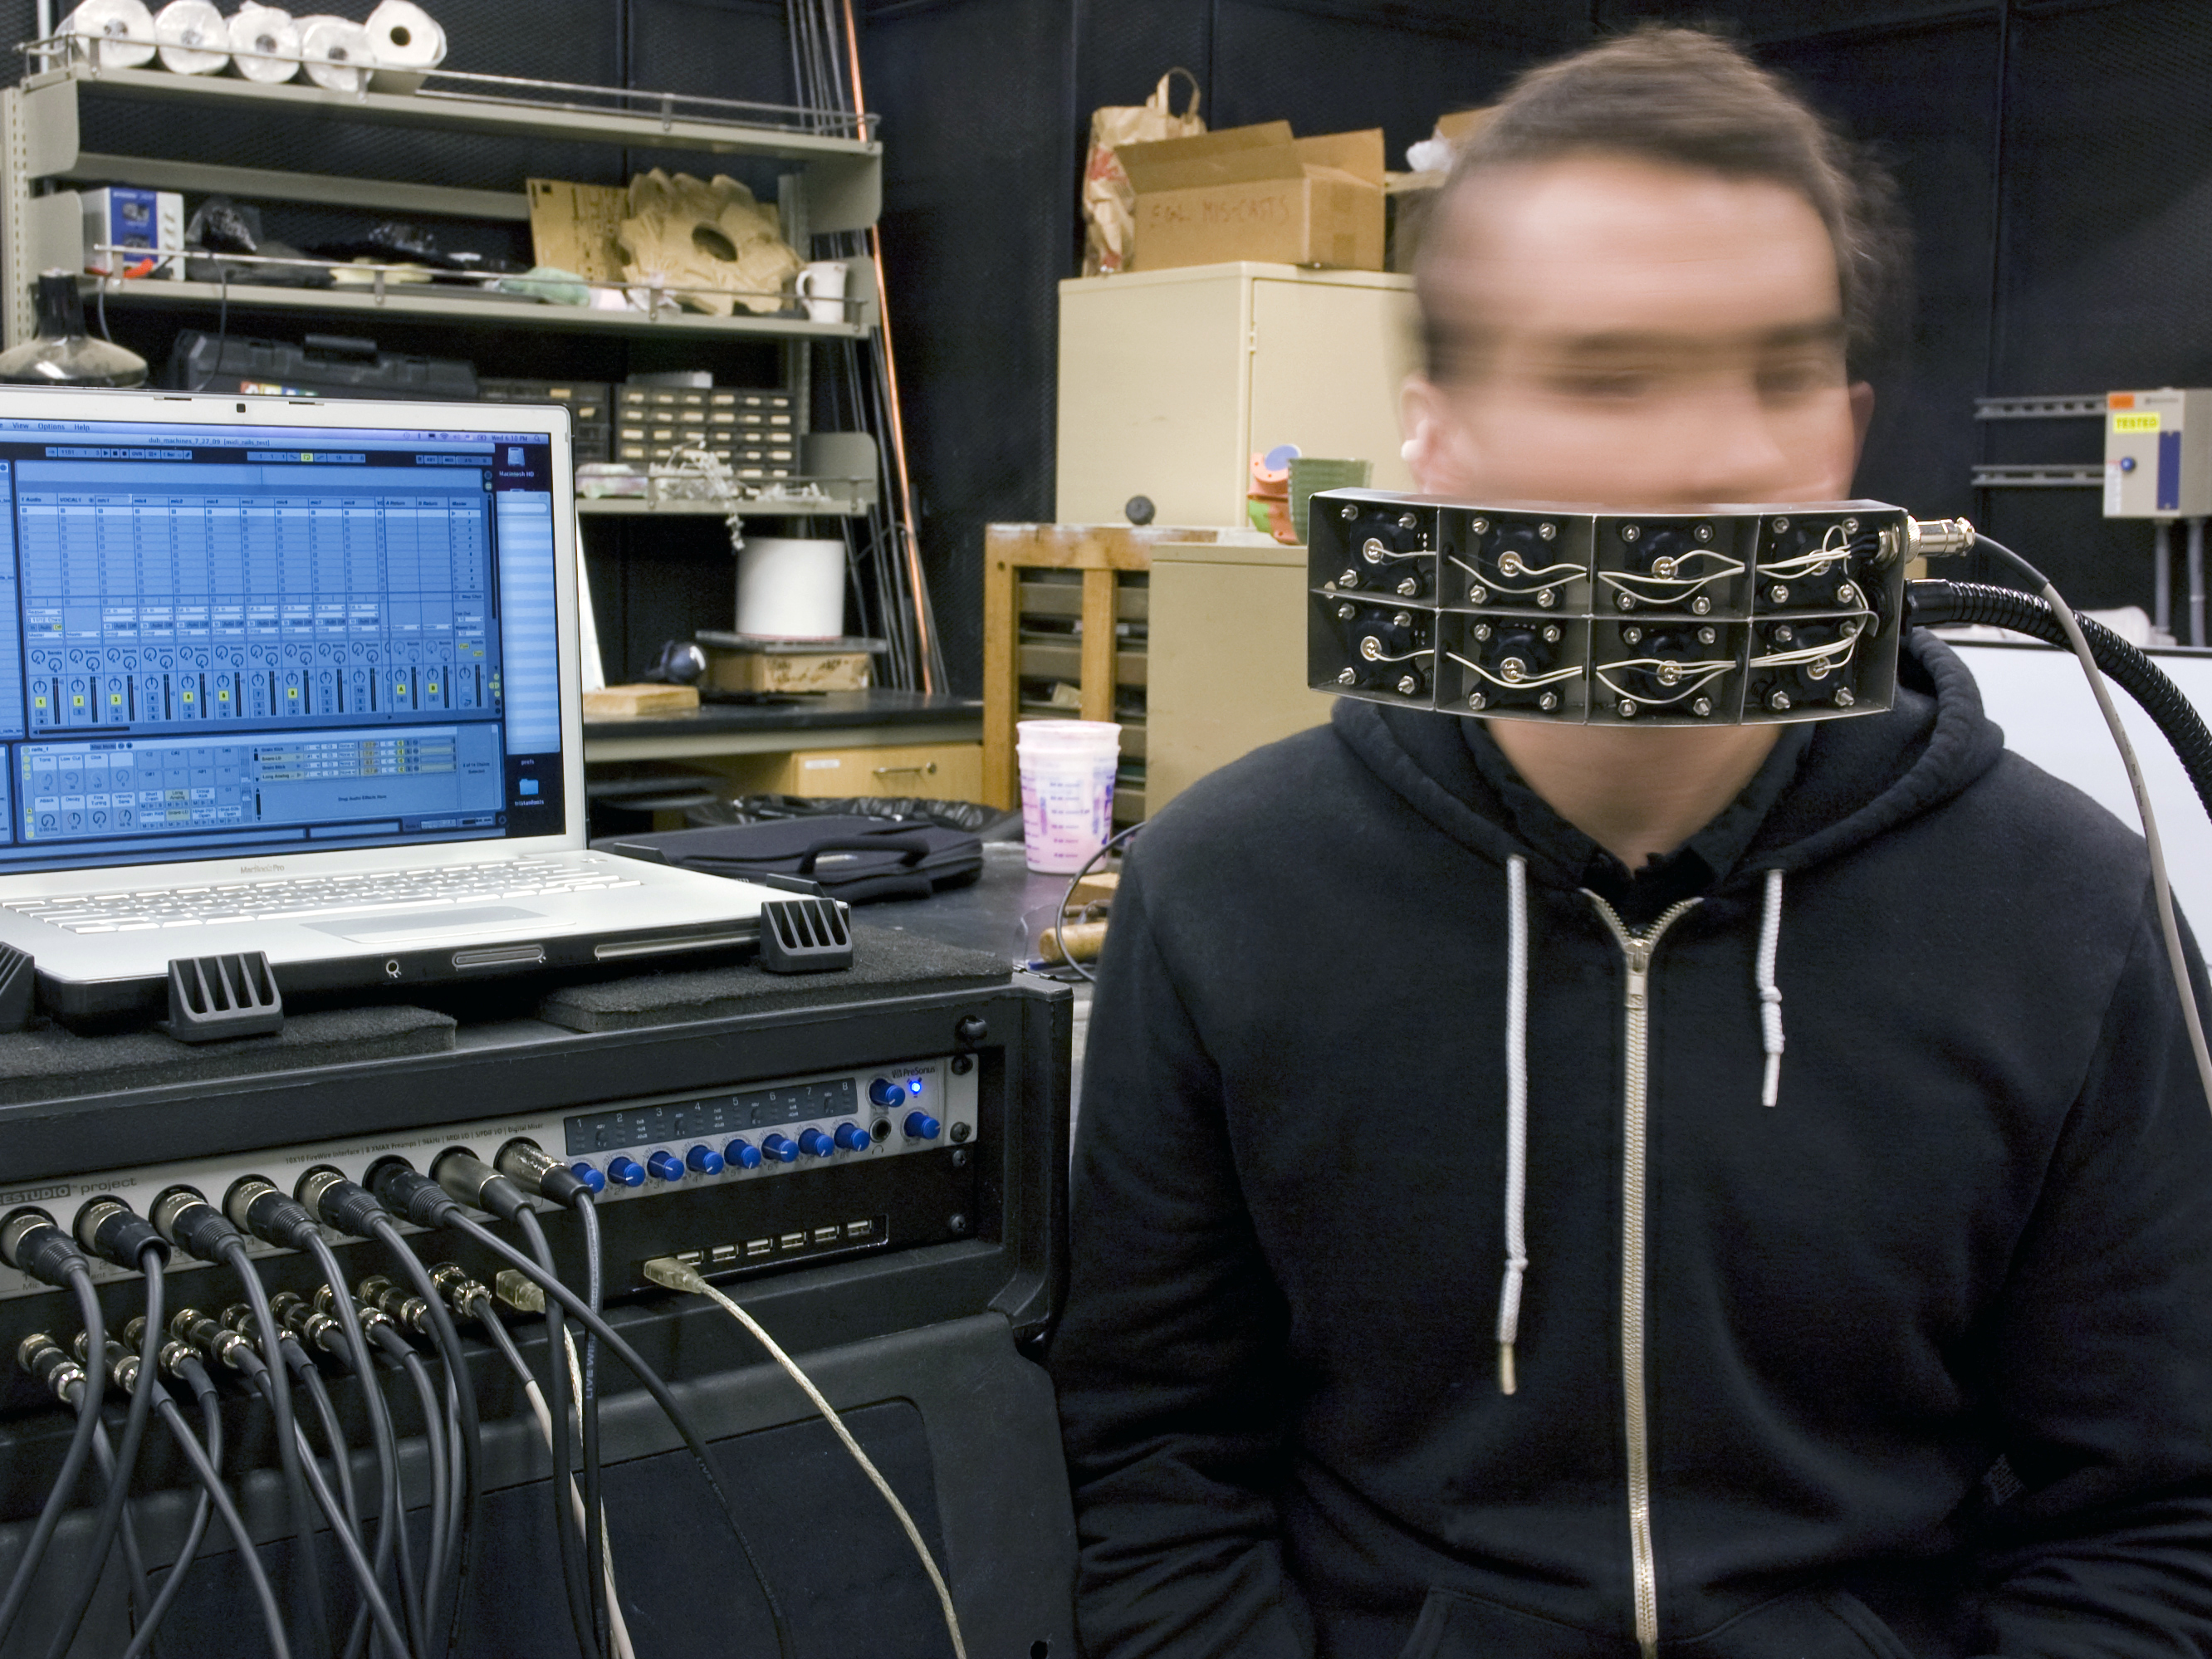
\includegraphics[width=1\textwidth]{headgear}
	\end{figure}
	
The circuit accompanying each microphone is simple and straightforward.  

		\begin{figure}[h!]
		  \caption{The schematic for each microphone wiring, from the MAKE article}
		  \centering
		    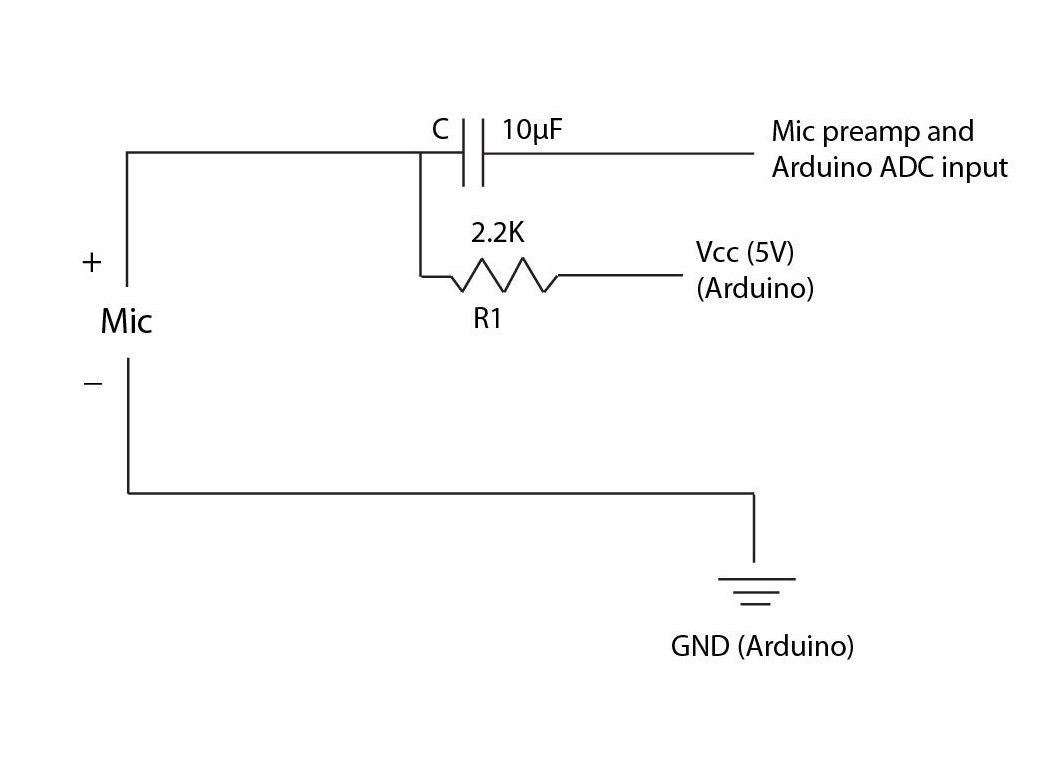
\includegraphics[width=1\textwidth]{micschem}
		\end{figure}
		
		The device fulfills once again two roles: it can act as a controller through the use of the Arduino system and its MIDI generating code (Shone uses the HIDuino firmware to facitilitate this, see next chapter), and it is used to provide sound to the rest of the system. 
	
	We see a trend in the systems being presented here: simple electronics, serving a specific purpose between exploration of a physical process (touching in the case of Cihan's \emph{Porcupine}, voice in the case of Shone).

	\emph{TRISTAN WILL SEND ARDUINO CODE FOR THE HEADGEAR FOR ANALYSIS}
	
The Headgear is not the main element of Shone's live setup, nor is it necessarily its centerpiece. However, through its dual operating mode, the sharing of its design on public platform such as MAKE magazine, and the relative simplicity of its inner workings, it serves as a good example of the few things needed by an accomplished fabricator and artist to make a compelling device. 

As can be expected in parallel with the rise of microcontrollers as interfaces for turning our environment into a source of control data, recent years have seen a number of initiatives turning accessible, general purpose computing devices into code-based synthesis engines. All these projects are the embodiment of their designer's curiosity, adapted to various degrees of interactivity for performance, composition or commercialisation. 

\subsection{Dan Snazelle, Snazzy FX}

Dan Snazelle is a recording engineer turned hardware designer. Although his relationship with musical electronics is mostly done through the design of analog electronics, he is one of the first to market an Arduino as the central piece of a synthesizer module. In doing so, Snazelle and his collaborator Darwin Grosse take advantage of the fast-paced communal activity of coding communities and the ability to sell a product even though there is enough information for people to build them from scratch. 

\paragraph{The Ardcore Eurorack-format module (2011, commercialized 2012)}

The Ardcore is in effect a reprogrammable lo-fidelity oscillator and control voltage generator packaged in a eurorack format and complemented by a set of freely available and editable programs. 

This project was developed by Darwin Grosse and Dan Snazelle. Darwin Grosse is a developper at Cycling `74, while Dan Snazelle is the owner and designer at Snazzy FX. Just like the Porcupine, the Ardcore documentation isn't all neatly packaged in a tutorial form, but a significant amount of  information is available for the curious. 

At the beginning of this project is Grosse's master's thesis at University of Colorado, Boulder. The document describes the first completed prototype and provides context, code examples, an overview of its possibilities, and detailed documentation of the collaboration process with Dan Snazelle. 

Of interest here is the information available to the tinkerer that might be interested in building their own homemade ardcore. 

Grosse's statement of purpose can be found in Appendix A of his thesis: 

\begin{quote}

	This specification provides the analog modular community with a standardized use of the Arduino microcontroller system, and will include a large number of example sketches (programs) that accomplish tasks within the modular world. Any Arduino user can utilize these specifications to create modules, control systems or computer interfaces, and will be able to use any programs that others may come up with.
	
	\end{quote}
	
	\citep{grosse2011}
		
		\begin{figure}[h!]
		  \caption{the first version circuit board, with an arduino nano}
		  \centering
		    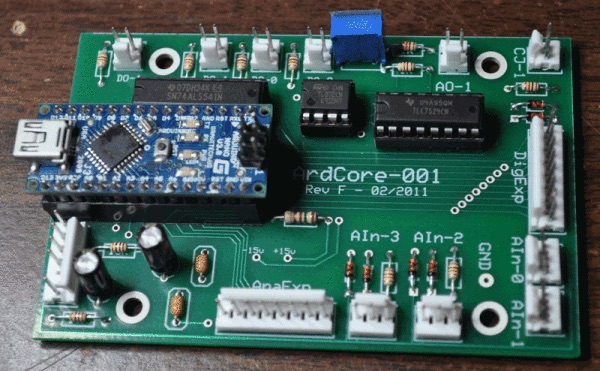
\includegraphics[width=1\textwidth]{ardcorev1}
		\end{figure}
		
		\begin{figure}[h!]
		  \caption{the first version synthesizer module, by Darwin Grosse}
		  \centering
		    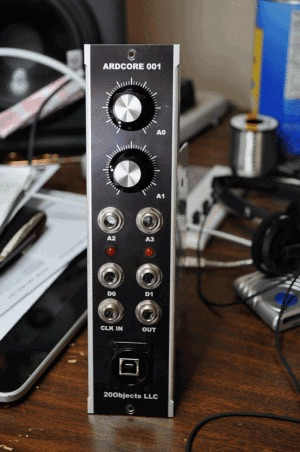
\includegraphics[width=1\textwidth]{ardcoremodule}
		\end{figure}
		
		\begin{figure}[h!]
		  \caption{the currently available ardcore, by Snazzy FX}
		  \centering
		    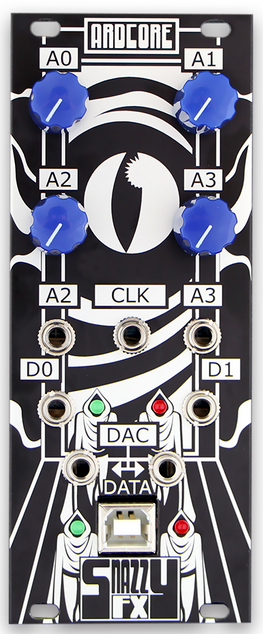
\includegraphics[width=.4\textwidth]{ardcoresnazzy}
		\end{figure}

Undertaking this project from scratch is somewhat more ambitious than any of the previous case studies. Because the arduino code is all shared on github, the software is not an issue, whichis in line with the practices of the arduino community. However, there doesn't seem to be any explicit tutorial or consolidated documentation for copying the hardware - although Grosse's thesis details the development and manufacture in much detail \citep[pp.21-31]{grosse2011}. 

		\begin{figure}[h!]
		  \caption{The schematic for the DAC section of the Ardcore, based around a TLC7524}
		  \centering
		    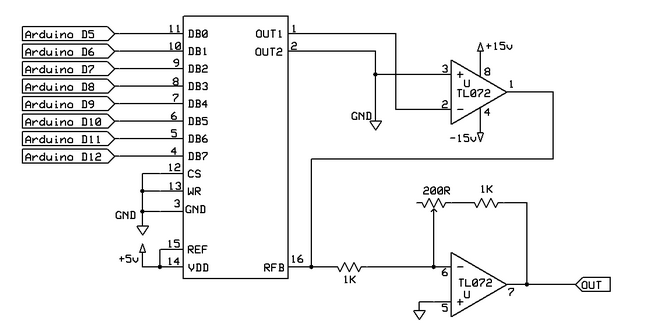
\includegraphics[width=1\textwidth]{ardcoredac}
		\end{figure}
		
		\begin{figure}[h!]
		  \caption{The circuit board layout for the first version Ardcore, by Darwin Grosse}
		  \centering
		    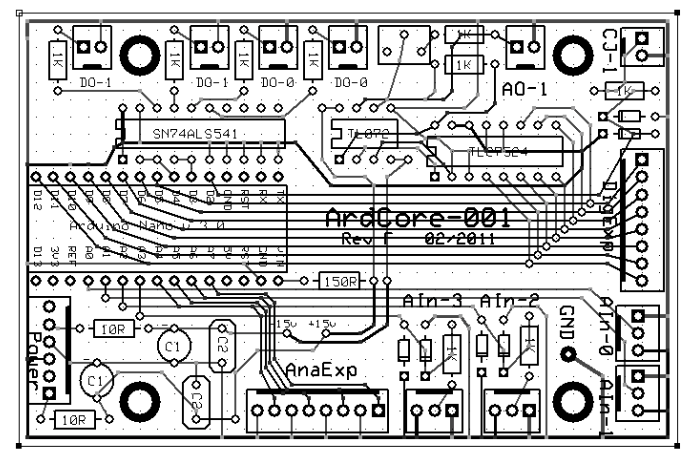
\includegraphics[width=1\textwidth]{ardcorepcb}
		\end{figure}

These documents do go a long way illustrating Grosse's preliminary design. Put briefly, the clock in is implemented on a digital input, and the analog out is done through eight other digital pins being connected to a TLC7524 digital to analog converter (DAC). All the voltage scaling for the module to be functional within the modular environment (Grosse chose the one volt per octave standard) was done through the use of a TL072 op amp circuit with an internal trimpot calibration. The Arduino processor (the Atmel documented previously) can now serve as an in/out device for audio signal (albei sampled at an 8 bit depth) and produce voltages conforming to other manufactured modules. 

As Grosse and Snazelle finalized the eurorack version of the module, it becomes clear that the focus is this device's ``lo-fi swiss army knife of modular'' versatilty. The two developers contribute actively to various repositories for newt module codes and application, with over sixty listed overall. 

The Arduino can be viewed as one of the driving force in making and tinkering today. Integrating in a nostalgia medium such as the modular synthesizer system is both beneficial for the life-span of both items and for maintaining the relevancy of a founding technology in electronic music. By placing both their future in the hands of an enthusiastic community, Grosse and Snazelle arguably guarantee both of their survivals.  

%https://github.com/eclectics/ardcore

%https://github.com/darwingrosse/ArdCore-Code

%\subsection{Tristan Perich and Loud Objects}

%Tristan Perich's dual approach to music hardware is most clearly divided between his highly predetermined solo work, and the more chaotic performances he presents with Loud Objects. As part of the latter trio, he solders their instrument - a set of microcontrollers - as part of the performance, making the piece a circuit in the most Tudorian sense of the idea. 

%As a composer, his work still relies on the binary output of microcontrollers, creating his ``one bit symphonies'' that have been presented as standalone pieces or along acoustic instruments in performances. 

%http://vagueterrain.net/journal19/loud-objects/01

%\subsection{Martin Howse}

%Martin Howse is a British artist residing in Berlin and teaching workshops all over the world. 

%Howse's esoteric psychogeophysics exploration is backed by a strong design and programming sense that's allowed him to turn some of his stranger ideas (booting a computer using noise from a metal stake in the ground as some of the BIOS code) into commercial products. 


%\paragraph{the dark interpreters}

%The dark interpreters is a series of three ARM processor based synthesizer: 


%http://1010.co.uk/manual.pdf

%https://github.com/microresearch/dark-interpreter

%http://syntone.fr/martin-howse-une-ecologie-des-signaux/

%http://www.1010.co.uk/org/darkint.html

%http://disnovation.net/bordeaux.html

%\section{Jessica Rylan, Flower Electronics}

%Rylan's circuit design practices present a common dilemna in art-oriented technology today first presented in chapter one: how to make something new and different with the same parts and similar circuits? 

%This disatisfaction with the seemingly uniform way modern electronics present audio and think of interfaces is presented as the motivation for a number of designs that wish to address this issue \citep[pp.139-155]{rodgers2010}. 

%Inspecting devices sold by her company Flower Electronics over their period of operation (late 2000's to early 2010's) only imprecisely informs one of how this might have been done. Enclosures are still standard Hammond aluminum, and the underlying circuits seem to reference mostly more unusual but known synthesis classics by Buchla, Serge, etc. A clear interest in chaotic oscillators is denoted, but even in that case, it seems difficult to break out of the VCO/VCF/VCA modular mold. 

%In some sense, Rylan's work is at its most compelling when it is presented in the context of her own history and musical practice. The personal synthesizer, started in 2004, is the aptly named tool she developed in this quest of alternative design. 

%\subsection{the personal synth}

%http://vagueterrain.net/journal19/jessica-rylan/01

%https://vimeo.com/20051159



\section{Sang Wook ``Sunny'' Nam: Mastering Studio}

Sang Wook Nam is a mastering engineer teaching at Dartmouth College and running a mastering studio at the time of this writing \citep{nam2015}. As a mastering engineer, Nam does not manufacture synthesis or signal processing hardware. His connection to music technology is presented here because it serves as a fitting conclusion to our lineup of hardware examples: even in professional, closed source environments, open design methods and its products are important. 

In visiting his studio, it appears that most items in his setup fall within standard categories of equipment: channel selectors, equalizers, amplifiers, high quality analog to digital / digital to analog converters, etc. However, it also becomes clear that all of this equipment is custom made to satisfy Nam's trained and precise ear. In an interesting and probably unintentional nod to David Tudor's mysteriously unlabeled devices, a noted amount of Nam's gear is minimally annotated. 

	\begin{figure}[h!]
	  \caption{Jacob's Well mastering desk}
	  \centering
	    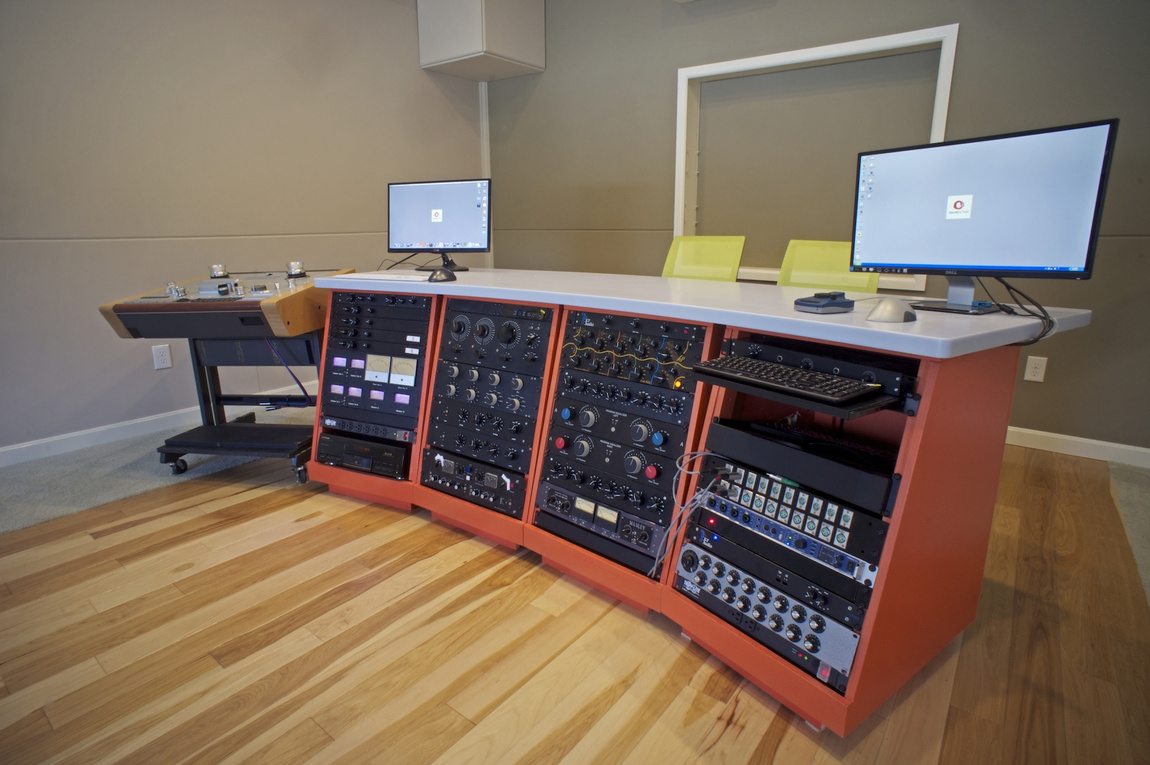
\includegraphics[width=1\textwidth]{sunnystudio}
	\end{figure}
	
Most of this equipment is designed, assembled and tested in collaboration with JCF audio's founder and owner, Joshua Florian \citep{florian2015}. After Nam and Florian worked together at LA's Mastering Lab, Nam came to value Florian's understanding of what they describe as ``yester-tech'' \citep{florian2015b}: older audio hardware circuit designs, usually discrete semiconductor or tube, that were used in high end recording and mastering studios along with the rise and heyday of major labels. A number of parts in Nam's current setup come from A\&R mastering studio, which he purchased when they closed down. 



This section does not contain a particular product description. However, the concept of ``yester-tech'' is, perhaps understatedly, at the bottom of the discussion on open-source hardware. Open-source is mostly defined in opposition to closed-source or proprietary information, the privacy of which is legally defended by its inventors and implementors. However, mu

For hardware, this information details the designs of devices, and in most technological economies, this intellectual property is legally protected by copyright, patents. Legally, these expire or have limitations allowing people today to rightfully build and sell their own version of, for example, the API 2520 that Nam mentions in his interview. 

The goals of including comments stemming from my discussion with Nam were simple: prove that secretive designers are still able to succesfully build businesses out of their expertise, expose their use of open-source designs, if any, and that simply taking from publicly available designs was itself a way to perpetuate its importance. In other words, open-source hardware design is a robust practice. 

\section{Design comments}

All these projects constitute a limited sample of the ideas driving innovation in the field of electronic music hardware. Through them, we've explored a significant amount of the space of possibilities defined in the first chapter by the components available. They  Primary sources range from highly formatted peer review journals to unstable forum posts, mired with dead links and noise.  

%Rather than trying 

% ---------------
% To incorporate in this chapter

\begin{unsortedStuff}	
\section*{(TO INCORPORATE)}
	\begin{itemize}
		\item 
	\end{itemize}
\end{unsortedStuff}
		
%Blank page to add written thoughts
\begin{optBlankSpace}
	\newpage
	\mbox{}
\end{optBlankSpace}

